\setlength{\footskip}{8mm}

\chapter{Introduction}


\section{Overview}

Data analysis is an very robust topic in the field of data science and encompasses the various mathematical functions. The functions are statistical in nature and are performed on the data obtained. The goal of data analytics is to support (or reject) the hypothesis which the data scientist postulates.
“ By processing a steady stream of real-time data, organizations can make time-sensitive decisions faster than ever before, monitor emerging trends, course-correct rapidly and jump on new business opportunities.” [BIG Data Analytics: A Framework for Unstructured Data Analysis pdf]

This paper tries to enlist most of the up-to-date techniques used by researchers and mathematicians to make sense of the data. Also the paper presents them in three groups of analytics.
But then there arises a question which is, why the need for data analytics ? Well, to answer that the paper proposes the literature from an article of Kdnuggets \shortcite{KDnuggets}.



According to Paul following are use cases  of data analytics :
1. Analytics powers our decisions – we do not need to guess while making bold new decisions, we should use the information from data at hand.
2. Your data analysis weighs down your opponent's argument.
3. Cut down on loss making ventures with data analytics.
4. Can be applied to all domains be it health-care, banking, marketing, sales, operations etc.
On the scenario when describing Data analytics it is very important to put the focus on Hypothesis.

Shown in the table \ref{tableDMusecase} is some business areas 


\begin{table}[H]
	\centering
%	\hskip-1.8cm
	\begin{tabular}{|p{4cm}|p{4cm}|l|}
		\hline
		\textbf{Application area} & \textbf{Applications} & \textbf{Specifics}\\
		\hline
		Insurance & Fraud detection & Identify claims meriting investigation\\
		\hline
		Telecom & Churn & Identify likely customer turnover\\
		\hline
		Telemarketing & On-line information & Aid telemarketers with easy data access\\
		\hline
		Human resource management & Churn & Identify potential employee turnover\\
		\hline
		\multirow{2}{4em}{Retail}  & Affinity positioning & Position product effectively\\
		& Cross-selling & Find more products for customers\\
		\hline
		\multirow{2}{4em}{Banking} & Customer relationship management & Identify customer value\\
		&& Develop programs to maximize revenue\\
		\hline
		Credit card management & Lift & Identify effective market segments\\
		& Churn & Identify likely customer turnover\\
		\hline
	\end{tabular}
	\caption{Data mining use cases}
	\label{tableDMusecase}
\end{table}
	
Figure \ref{fig:data-analytics} is a view of the data analytics with respect to the main fields.

\begin{figure}[H]
	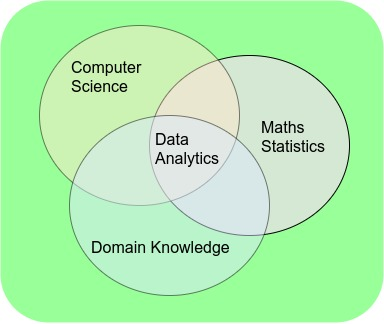
\includegraphics[scale = 0.8]{figures/FlowChart.jpg}
	\centering
	\caption{Data Analytics}
	\label{fig:data-analytics}
\end{figure}
\FloatBarrier

\section{Why Analytics for financial institutions ?}
According to a joint research study, by Boston Consulting Group and Morgan Stanley with analytics professionals, it was reveled that the financial institutions lagged behind other verticals in the use of data analytics~\shortcite{BCGanalytics2017} and it is shown in figure~\ref{fig:da_digitization}. One of the findings of the research was that FI's are investing a lot of capital, an estimated total of about \textdollar1bn. In addition it was found that for near term value creation the FI's expected data analytics to optimize customer acquisition, customer retention, operational efficiency, and risk mitigation.
\newline
\newline
\begin{figure}[H]
	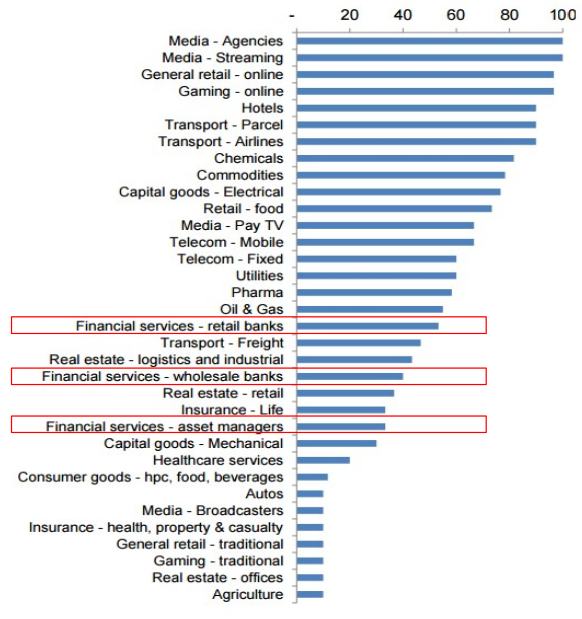
\includegraphics[scale = 0.7]{figures/DA_used_verticals.png}
	\caption{Reprinted from the Morgan Stanley Digitization Index ranks }
	\label{fig:da_digitization}
\end{figure}
\FloatBarrier

\section{State of analytics in financial companies}
From the survey of FI's, a mix of interviewees representing payment companies, service providers, insurance, commercial banks, BCG made some interesting discoveries. It was found that most organizations have invested in analytics techniques to generate market perceptions. Some of the most used were those of social media, log, text and location analytics as shown in figure~\ref{fig:da_capabilities}.

\begin{figure}[H]
	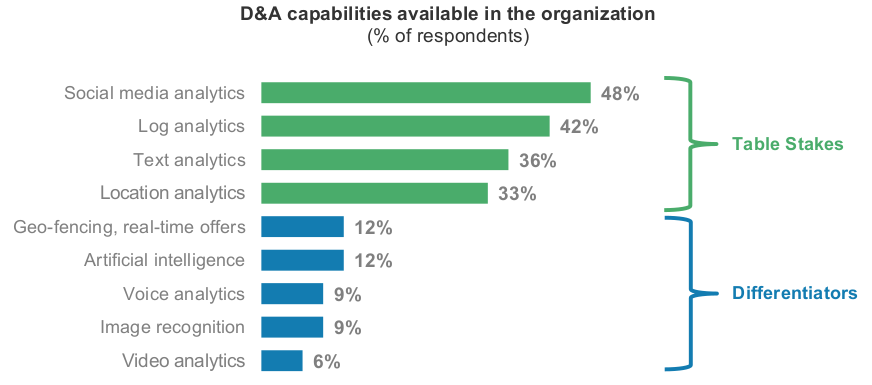
\includegraphics[scale = 0.5]{figures/DA_capabilities.png}
	\caption[Da capablities]{Reprinted from the work of Boston consulting group  }
	\label{fig:da_capabilities}
\end{figure}
\FloatBarrier

Researchers have highlighted that most of the interviewees claimed that institutions are yet to make substantial gain from investments in analytics. They identified that companies can make gains from automation and digitization of manual processes. Additionally, it was noted that financial institutions are adopting digital processes to automate data collection for KYC (Know Your Customer) service and Anti-money laundering 
%\newline
%\newline
Customers are loyal consumers of products, which give value for their monetary investments. Big institutions tend to over look the need for value creation and focus their analytics and metrics to improve profit \shortcite{Reichheld1996}. In the HBR report Reichheld makes certain  observations that customers of large companies witness degrading value standards and secondly increasing rate of customer churn is a good variable to predict cash flow from consumer to company. He also noted that companies can replace old customer with new ones but the profits are lower as cost of induction is high.


	

2. Categories in data analytics :
There are three basic categories viz. Descriptive, Predictive and Prescriptive. The methods and techniques are described further in the paper, and they are classified into the above.

2.1 Descriptive Analytic techniques: The sole purpose of using the methods in this category would be to describe the Hypothesis. Descriptive analytics or data mining are at the bottom of the big data value chain, but they can be valuable for uncovering patterns that offer insight. A simple example of descriptive analytics would be assessing credit risk; using past financial performance to predict a customer’s likely financial performance. Descriptive analytics can be useful in the sales cycle, for example, to categorize customers by their likely product preferences and sales cycle.

To summarize data into meaningful charts and reports, for example, about budgets, sales, revenues, or cost. They allow managers to obtain standard and customized reports, and drill down into the data and to make queries to understand the impact of an advertising campaign, for example, review business performance to find problems or areas of opportunity, and identify patterns and trends in data. Typical questions that descriptive analytics help answer are: How much did we sell in each region? What was our revenue and profit last quarter? How many and what types of complaints did we resolve? Which factory has the lowest productivity? Descriptive analytics also help companies to classify customers into different segments, which enable them to develop specific marketing campaigns and advertising strategies. [1]

There are two main approaches to apply in this topic Data warehousing and Visual analytics with reporting.

2.2 Predictive analytic techniques : Predictive analytics use big data to identify past patterns to predict the future. For example, some companies are using predictive analytics for sales lead scoring. Some companies have gone one step further use predictive analytics for the entire sales process, analyzing lead source, number of communications, types of communications, social media, documents, CRM data, etc. Properly tuned predictive analytics can be used to support sales, marketing, or for other types of complex forecasts.


2.3 Prescriptive analytic techniques : Prescriptive analytics is really valuable, but largely not used. According to Gartner, 13 percent of organizations are using predictive but only 3 percent are using prescriptive analytics. Where big data analytics in general sheds light on a subject, prescriptive analytics gives you a laser-like focus to answer specific questions. For example, in the healthcare industry, you can better manage the patient population by using prescriptive analytics to measure the number of patients who are clinically obese, then add filters for factors like diabetes and LDL cholesterol levels to determine where to focus treatment. The same prescriptive model can be applied to almost any industry target group or problem.


There is yet another classification of Analytics tools on the basis of the generation ie. Traditional vs Advanced.[1] [1 - https://rapidminer.com/summarizing-differences-business-intelligence-advanced-analytics/]

Traditional analytics employ visualizations like graphs, charts (pie, bar), infographics etc., querying, reporting, scorecards and OLAP. They tend to answer the Descriptive analytics type of questions. Generally used in Business Intelligence softwares, just query from existing data and display intuitive infographics, the user deciphers the data. The process of the business intelligence is generally termed as reactive.
Tools in consumer market WebFOCUS InfoAssist OLAP, IBM Cognos, Netweaver, Microstrategy Intelligence Server, andara Balanced Scorecard, BSC designer and any SQL relational database like Oracle, Microsoft Sql Server.
1. OLAP
2.Dashboards
3. Scorecards
4. KPI’s

Advanced analytics, on the other hand go beyond the traditional techniques. They use modeling, optimization, statistics methods to discover the future and predict an outcome. The softwares may also be termed as decision support systems or expert systems as they generate possible deductions. User could use the help and substantiate their own judgments. The process in this category is termed as proactive.
Methods used in advanced analytics are: predictive modeling, Statistical analysis, Simulation and Optimization, Text mining, Data mining, Multimedia mining, Descriptive modeling.
Tools in the consumer market are Powerpivot, Tableau, Qliksense, Yellowfin, etc.
1. Statistical Methods
2. Text Mining
3. Data Mining
4. Multimedia mining
5. Simulation
6. Optimization


3. Fields and Domains of application :



\section{Objectives}

The overall objective of the study report is to understand the major methods, techniques and tools adopted by financial institutions to perform data analytics.



%\section{Thesis Outline}

%The organization of this dissertation is as follows:
%\begin{itemize}
%	\item In Chapter \ref{ch:literature-review}, the literature review is explored.
%	\item In Chapter \ref{ch:methodology}, the methodology is proposed.
%\end{itemize}

%In Chapter \ref{ch:results}, I present the experimental results.
%Finally, in Chapter \ref{ch:conclusion}, I conclude my thesis.

\FloatBarrier
